\documentclass[a4paper,12pt]{article}
\usepackage{graphicx}

\begin{document}
\title{SCIO}
\maketitle

\section*{Data preparation}
The raw data consists on two dataframes, SCIO and DXA. The former contains the results of all the SCIO measurements, plus additional feature information for each measurement. The latter contains the results from the DXA measurements. In detail:\\

SCIO columns:
\begin{itemize}
	\item folio: woman identifier.
	\item mama: breast identifier (right, left, left2).
	\item ubicacion: location of SCIO shot (3pm, 6pm, 9pm, 12pm, pezon).
	\item feature columns: BMI, weight, height, fitzpatrick color, nipple radius, bra size, age.
	\item spectrum columns: 331 SCIO normalized measurements for 331 different spectrum values.
\end{itemize}

DXA columns:
\begin{itemize}
	\item folio: woman identifier.
	\item mama: breast identifier (right, left, left2).
	\item DXA density: DXA density measurement.
\end{itemize}

After merging both tables we get
\begin{itemize}
	\item 197 folios.
	\item 3 breast per folio.
	\item 5 locations per breast.
	\item 3 spectrum measurements per location
\end{itemize}

\section*{Variability within left breast measurements}
We examine now how much does the variability of the SCIO measurements can be attributed to differences in the breast locations, and how much is due the imprecisions of the instrument. The following histogram illustrates the percentage variation between the two measurements of the left breast for each folio, and the percentage variation of a folio with respect to the average.

More in concrete:


\begin{figure}[ht!]
	\centering
	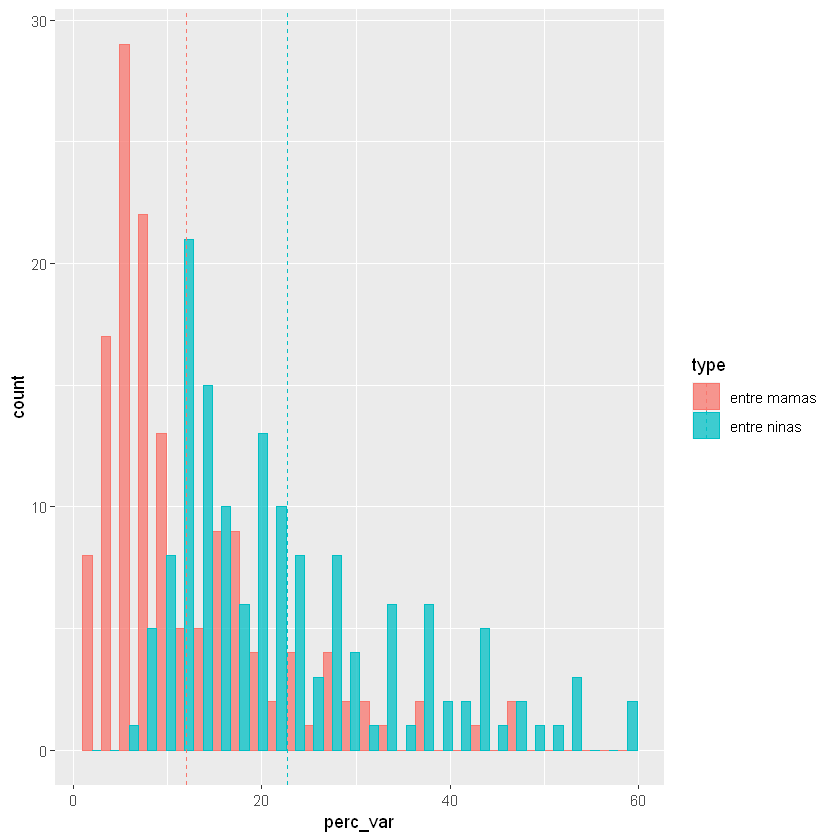
\includegraphics[trim={0 0cm 0cm 0}, clip, scale=0.55]{figures/variability_histogram.png}
	\caption{.} 
	\label{fig:abt_vs_base}
\end{figure}

Around 30\% of folios have a left breast variation that is indistinguishable from the variation between folios.  From now on, we drop these folios.

\section*{Analysis}
The following is the distribution of spectrum values per breast by BMI of folio:
\begin{figure}[ht!]
	\centering
	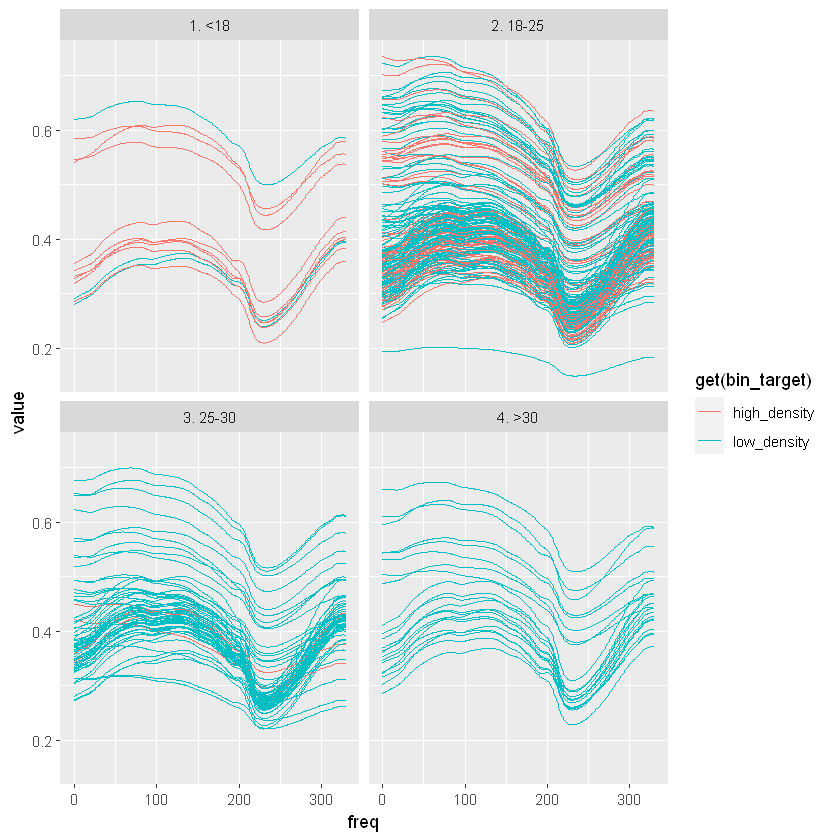
\includegraphics[trim={0 0cm 0cm 0}, clip, scale=0.55]{figures/scio_by_bmi.png}
	\caption{.} 
	\label{fig:abt_vs_base}
\end{figure}

\end{document}

